\documentclass{beamer}

\usetheme{Madrid}
\usepackage[utf8]{inputenc}
\usepackage[T1]{fontenc}
\usepackage[american]{babel}
\usepackage{graphicx}
\usepackage[nolist,nohyperlinks]{acronym}
\usepackage{amsmath}
\usepackage{amsthm}
\usepackage{amssymb}
\usepackage{mathpartir}
\usepackage{adjustbox}
\usepackage{xcolor, colortbl}
\usepackage{soul}
\usepackage{wrapfig, tabularx}
\usepackage{adjustbox, listings}
\usepackage{tikz}

\usetikzlibrary{arrows}

\definecolor{shyellow}{rgb}{.9, .8, .2}
\definecolor{shpurple}{rgb}{.9, .6, .8}

\newcommand{\hlmod}[1]{{%
    \sethlcolor{shyellow}\hl{#1}}%
}

\newcommand{\hlnew}[1]{{%
    \sethlcolor{shpurple}\hl{#1}}%
}


\acrodef{FOP}[FOP]{Feature Oriented Programming}
\acrodef{ITP}[ITP]{Interactive Theorem Prover}
\acrodef{FJ}[FJ]{Featherweight Java}
\acrodef{FFJ}[FFJ]{Feature Featherweight Java}
\acrodef{FFJ+}[FFJ\textsubscript{+}]{Overhaul Feature Featherweight Java}


\newcommand{\cdecl}[6]{\texttt{class #1 extends #2 \{\={#3} \={#4}; #5 \={#6}\}}}
\newcommand{\crefine}[6]{\texttt{refines class #1 \{\={#2} \={#3}; #4 \ensuremath{\mathtt{\overline{#5}~\overline{#6}\}}}}}
\newcommand{\mdecl}[5]{\texttt{#1 #2 (\ensuremath{\mathtt{\overline{#3}~\overline{#4}}}) \{return #5;\}}}
\newcommand{\mrefine}[5]{\texttt{refines #1 #2 (\ensuremath{\mathtt{\overline{#3}~\overline{#4}}}) \{return #5;\}}}


\title[Mechanization and Overhaul of FFJ]{Mechanization and Overhaul of Feature Featherweight Java with Coq}

\author{Pedro da C. Abreu Jr.}

\institute[UnB]
{
	Universidade de Brasilia 
}

\date{08 de Agosto, 2017}

\subject{Formalização de Linguagens de Programação}


% Let's get started
\begin{document}
	
	\begin{frame}
		\titlepage
	\end{frame}
	
	%\begin{frame}{Roteiro}
		%\tableofcontents
	%\end{frame}

    \begin{frame}{Mecanização}
        \begin{itemize}
            \item Mecanizar significa provar teoremas com a assistência do computador.
                \begin{itemize}
                    \item<2-> Automaticamente;
                    \item<3-> Iterativamente.
                \end{itemize}
        \end{itemize}
    \end{frame}

    \begin{frame}{Provadores Iterativos de Teoremas}
        
\includegraphics[width=\textwidth, height=\textheight]{itp_logos}
    \end{frame}

    \begin{frame}{Por que mecanizar?}
        \begin{itemize}
            \item Aplicações de segurança critica: Bugs são inaceitáveis
            \begin{itemize}
                \item Controladores de Avião
                \item Equipamentos Médicos
                \item Carros
            \end{itemize}
        \item<2-> A medida que o software e o hardware crescem dificulta encontrar
            bugs através de testes.
        \item<3-> Bugs encontrados tardiamente são caros.
            \only<3->\footnote{Fonte: The Economic Impacts of Inadequate Infraestructure for Software Testing}
        \end{itemize}
    \end{frame}

    %% \begin{frame}{Bugs são caros}
    %%     \centering
    %%         Custo Relativo para Corrigir Defeitos Encontrados em
    %%         Diferentes Fases do Desenvolvimento de Software.\footnote{Fonte: The Economic Impacts of Inadequate Infraestructure for Software Testing}\\

    %%         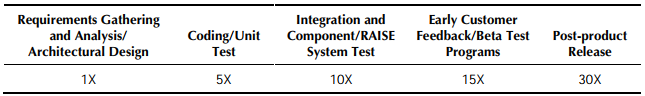
\includegraphics[width=\textwidth]{custo_bug}
    %% \end{frame}

    \begin{frame}{O que é feature?}
        \centering
        \begin{block}{Feature}
            `A feature is a unit of functionality of a software system
            that satisfies a requirement, represents a design decision, and provides a potential
            configuration option.' - S. Apel \& K. Kastner
        \end{block}
    \end{frame}

    \section{Feature Oriented Programming}
    \begin{frame}{Feature Oriented Programming}{Software Product Line}
        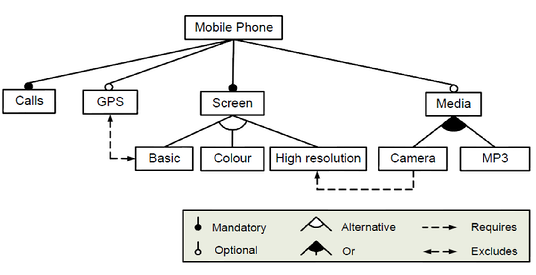
\includegraphics[width=\textwidth]{spl-ex}
    \end{frame}

    \begin{frame}{Objetivo}
        \centering
        Mecanizar Feature Featherweight Java 
    \end{frame}

    \section{Featherweight Java}
    \begin{frame}{Featherweight Java}{Sintaxe Abstrata}
        \begin{table}[!ht]
            \centering
            \begin{tabular}{lr}
                \texttt{CD}~::= \hfill \textit{class declarations:}\\
                \quad \cdecl{C}{D}{C}{f}{K}{M} \\  \\
                \texttt{K}~::=  \hfill\textit{constructor declarations:}\\
                \quad \texttt{C(\={C}~\={f})\{super(\={f});~this.\={f}=\={f};\}}\\\\
                \texttt{M}~::= \hfill\textit{method declarations:}\\
                \quad \mdecl{C}{m}{C}{x}{e} \\ \\
            \end{tabular}
            \quad
            \label{abstractsyntax}
        \end{table}
        %
    \end{frame}

    \begin{frame}{Featherweight Java}{Sintaxe Abstrata}
        \begin{table}[!ht]
            \centering
            \begin{tabular}{lr}
                \texttt{e}~::= \hfill \textit{expressions:}\\
                \quad \texttt{x} \\ 
                \quad \texttt{e.f} \\
                \quad \texttt{e.m(\={e})} \\
                \quad \texttt{new~C(\={e})} \\
                \quad \texttt{(C)e} \\ \\
                \texttt{v}~::= \hfill \textit{values:}\\
                \quad \texttt{new~C(\={e})}
            \end{tabular}
        \end{table}
    \end{frame}

	\section{Subtype}
    \begin{frame}{Featherweight Java}{Relação de Subtipo}
        \begin{table}
            \begin{tabular}{c@{\qquad}c@{\qquad}c}
                \inferrule{ }{\texttt{C~<:~C}} & 
                \inferrule{\texttt{C <: D} \qquad \texttt{D <: E}}
                {\texttt{C~<:~E}} &
                \inferrule{\texttt{class~C~extends~D~\{~\ldots~\}}}
                {\texttt{C~<:~D}} \\
            \end{tabular}
        \end{table}
    \end{frame}


    \begin{frame}{\only<2->{Feature} Featherweight Java}{\only<1>{Relação de Subtipo} \only<2->{Refinement Chain}}
        \centering

        \begin{tikzpicture}
            \centering

            \tikzset{vertex/.style = {shape=circle,draw,minimum size=1.5em}}
            \tikzset{edge/.style = {->,> = latex'}}
            % vertices
            \node[vertex] (a) at  (0,0) {$A$};
            \uncover<2->{\node[vertex] (a1) at  (0,-2) {$A_1$};}
            \uncover<2->{\node[vertex] (a2) at  (0,-4) {$A_2$};}
            \node[vertex] (b) at  (2,0) {$B$};
            \node[vertex] (c) at  (4,0) {$C$};
            \uncover<2->{\node[vertex] (c1) at  (4,-2) {$C_1$};}
            \uncover<2->{\node[vertex] (c2) at  (4,-4) {$C_2$};}
            \uncover<2->{\node[vertex] (c3) at  (4,-6) {$C_3$};}
            \node[vertex] (d) at  (6,0) {$Obj$};
            %edges
            %\draw[edge] (a) to (b);
            \path[->] (a) edge node [above] {$\mathtt{<:}$} (b);
            \path[dashed, ->]<2-> (a1) edge node [left] {} (a);
            \path[->]<2-> (a2) edge node [left] {\only<3->{pred}} (a1);
            \draw[edge] (b) to (c);
            \path[dashed, ->]<2-> (c1) edge node [left] {} (c);
            \path[->]<2-> (c2) edge node [left] {} (c1);
            \path[->]<2-> (c3) edge node [left] {} (c2);
            \draw[edge] (c) to (d);
            \path[->]<3-> (a) edge[out=160, in=180, red] node [left] {last} (a2);
        \end{tikzpicture}

    \end{frame}


    \section{Feature Featerweight Java}
    \begin{frame}{Sintaxe Abstrata}
        \begin{table}[!ht]
            \centering
            \begin{tabular}{lr}
                \hlnew{\texttt{R}~::=} \hfill \textit{refinement names:} \\
                \quad \hlnew{\texttt{C@feat}} \\ \\
                \hlmod{\texttt{CR}~::=} \hfill \textit{class refinements:}\\
                \quad \hlmod{\texttt{refines class R \{\={C} \={f}; KD \={M} \={MR}\}}} \\ \\
                \texttt{KD}~::= \hfill\textit{constructor refinements:} \\
                \quad \texttt{refines~C(\={E}~\={h}, \={C} \={f})\{original(\={f}); this.\={f}=\={f};\}} \\\\
                \texttt{MR}~::= \hfill \textit{method refinements:}\\
                \quad \mrefine{C}{m}{R}{x}{e} \\ \\
            \end{tabular}
            \quad
            \label{abstractsyntax}
        \end{table}
        %
    \end{frame}

	\section{Lookup Functions}

    \begin{frame}{Field Lookup}
        \begin{table}[ht!]
            \centering
            \begin{tabular}{c}
                $fields~$\texttt{Object}$=\bullet$ \\
                \\
                \inferrule{\texttt{class C extends {\only<3>{\color{red}}D} \{{\only<3>{\color{red}}\=C \=f}; K \=M\}} \qquad 
                        \only<2>{\color{red}}\neg\textit{last}~\texttt{C}}
                    {fields~\texttt{C}=fields~\texttt{{\only<3>{\color{red}}D}, {\only<3>{\color{red}}\={C} \={f}}}} \\
                \\
                \inferrule{\texttt{class C extends D \{\=C \=f; K \=M\}}}
                    {fields~\texttt{C}=fields~\texttt{D, \={C} \={f},}~\only<4>{\color{red}}fields_R~(last~\texttt{C})}\\
                \\
            \end{tabular}
        \end{table}

    \end{frame}

    \begin{frame}{Field Lookup (Refinement)}
        \begin{table}[ht!]
            \centering
            \begin{tabular}{c}
                \inferrule{\texttt{refines R \{\=C \=f; KR \=M \={MR}\}} \qquad
                        \only<2>{\color{red}}\neg pred~\texttt{R}}
                    {fields_R~\texttt{R}~=~\texttt{\=C \=f}} \\
                \\
                \inferrule{\texttt{refines R \{{\only<3>{\color{red}}\=C \=f}; KR \=M \={MR}\}}}
                    {fields_R~\texttt{R}=fields_R~({\only<3>{\color{red}}pred~\texttt{R}}), \only<3>{\color{red}}\texttt{\={C} \={f}}}\\
            \end{tabular}
        \end{table}
    \end{frame}



    \newcommand{\mtype}[2]{\ensuremath{mtype~(\texttt{#1},\texttt{#2})}}
    \newcommand{\mtyper}[2]{\ensuremath{mtype_R~(\mathtt{#1},\mathtt{#2})}}
    \newcommand{\mrettype}[2]{\ensuremath{\mathtt{\overline{#1}}}~\rightarrow~\mathtt{#2}}

    \begin{frame}{Method Type Lookup}
        \begin{table}[h!]
            \begin{tabular}{c}
                \inferrule{\cdecl{C}{D}{C}{f}{K}{M} \qquad 
                \only<5>{\color{red}}\mdecl{{\only<6>{\color{red}}B}}{m}{{\only<6>{\color{red}}B}}{x}{e} \in \texttt{\={M}} \\
                \only<2,4-5>{\color{red}}\neg\mtyper{m}{\mathnormal{last}~C}}
                {\mtype{m}{C}~=~\mrettype{\only<6>{\color{red}}B}{\only<6>{\color{red}}B}} \\ 
                \\
                \inferrule{\cdecl{C}{{\only<8>{\color{red}}D}}{C}{f}{K}{M} \qquad 
                    \only<7>{\color{red}}\texttt{m}\notin~\texttt{\={M}} \\\\
                    \only<2,4,7>{\color{red}}\neg\mtyper{m}{\mathnormal{last}~C}}
                {\mtype{m}{C}~=~\mtype{m}{\only<8>{\color{red}}D}} \\
                \\
                \inferrule{\cdecl{C}{D}{C}{f}{K}{M}}
                {\mtype{m}{C}~=~\only<2-3>{\color{red}}\mtyper{m}{\mathnormal{last}~C}} \\

            \end{tabular}
            \quad\\
            \label{mtypelookup}
        \end{table}
    \end{frame}


    \begin{frame}{Method Type Lookup (Refinement)}

    \begin{table}[h!]
	\centering
	\begin{tabular}{c}
        \inferrule{\crefine{R}{C}{f}{KR}{M}{MR} \qquad 
                \only<2>{\color{red}}\mdecl{{\only<3>{\color{red}}B}}{m}{{\only<3>{\color{red}}B}}{x}{e} \in \texttt{\={M}}}
                {\mtyper{m}{R}~=~\mrettype{\only<3>{\color{red}}B}{\only<3>{\color{red}}B}} \\ \\
        \inferrule{\crefine{R}{C}{f}{KR}{M}{MR} \qquad 
                \only<4>{\color{red}}\texttt{m} \notin \texttt{\={M}} \\
                \only<4>{\color{red}}\mrefine{{\only<5>{\color{red}}B}}{m}{{\only<5>{\color{red}}B}}{x}{e} \in \overline{\texttt{MR}}}
                {\mtyper{m}{R}~=~\mrettype{\only<5>{\color{red}}B}{\only<5>{\color{red}}B}} \\ \\
        \inferrule{\crefine{R}{C}{f}{KR}{M}{MR} \\\\
                \only<6>{\color{red}}\texttt{m} \notin \texttt{\={M}} \quad
                \only<6>{\color{red}}\texttt{m} \notin \overline{\texttt{MR}}}
                {\mtyper{m}{R}~=~\mtyper{m}{\only<6>{\color{red}}\mathnormal{pred}~P}} \\ 
    \end{tabular}
    \end{table}
    \end{frame}
    \newcommand{\mbody}[2]{\ensuremath{mbody~(\mathtt{#1},\mathtt{#2})}}
    \newcommand{\mbodyr}[2]{\ensuremath{mbody_R~(\mathtt{#1},\mathtt{#2})}}
    \newcommand{\mretbody}[2]{\texttt{\={#1}}\ensuremath{.}\texttt{#2}}


    \begin{frame}{Method Body Lookup}
        \begin{table}
            \begin{tabular}{c}
                \inferrule{\cdecl{C}{D}{C}{f}{K}{M} \qquad 
                \mdecl{B}{m}{B}{x}{e} \in \texttt{\={M}} \\\\
                \neg\mbodyr{m}{\mathnormal{last}~C}}
                {\mbody{m}{C}~=~\mretbody{x}{e}} \\ 
                \\
                \inferrule{\cdecl{C}{D}{C}{f}{K}{M} \qquad 
                    \texttt{m}\notin~\texttt{\={M}} \\\\
                    \neg\mbodyr{m}{\mathnormal{last}~C}}
                {\mbody{m}{C}~=~\mbody{m}{D}} \\
                \\
                \inferrule{\cdecl{C}{D}{C}{f}{K}{M}}
                {\mbody{m}{C}~=~\mbodyr{m}{\mathnormal{last}~C}} \\

            \end{tabular}

        \end{table}
    \end{frame}

    \begin{frame}{Method Body Lookup (Refinement)}

        \begin{table}[h!]
            \centering
            \begin{tabular}{c}
                \inferrule{\crefine{R}{C}{f}{KR}{M}{MR} \qquad 
                \mdecl{B}{m}{B}{x}{e} \in \texttt{\={M}}}
                {\mbodyr{m}{R}~=~\mretbody{x}{e}} \\ \\
                \inferrule{\crefine{R}{C}{f}{KR}{M}{MR} \qquad 
                \texttt{m} \notin \texttt{\={M}} \\
                \mrefine{B}{m}{B}{x}{e} \in \overline{\texttt{MR}}}
                {\mbodyr{m}{R}~=~\mretbody{x}{e}} \\ \\
                \inferrule{\crefine{R}{C}{f}{KR}{M}{MR} \\\\
                \texttt{m} \notin \texttt{\={M}} \quad
                \texttt{m} \notin \overline{\texttt{MR}}}
                {\mbodyr{m}{R}~=~\mbodyr{m}{\mathnormal{last}~P}} \\ 
            \end{tabular}
        \end{table}
    \end{frame}

    \begin{frame}{Tipagem}
        \centering
        \only<1->{$\Gamma \vdash e: C$}

        \only<2->{
        $\Downarrow$

        $a: A, b: B, ..., x: X \vdash e: C$}
    \end{frame}

	\begin{frame}{Regras de Tipagem}
		\begin{table}[h!]
			\centering
			\def\arraystretch{3}
			\adjustbox{max height=\dimexpr\textheight-5.5cm\relax, max width=\textwidth}{
			\begin{tabular}{cr}
				$\Gamma \vdash x:\Gamma(x)$& (T-Var)\\
				
				\inferrule{\Gamma \vdash e_{0}:C_{0}\qquad fields~(C_{0})=\overline{C}\
					\overline{f}}
				{\Gamma \vdash e_{0}.f_{i}:C_{i}} & (T-Field)\\
				
				\inferrule{\Gamma \vdash e_{0}:C_{0}\qquad
					mtypes~(m,~C_{0})=\overline{D}\rightarrow C\qquad \Gamma \vdash
					\overline{e} : \overline{C} \qquad \overline{C}~<:~\overline{D}}
				{\Gamma \vdash e_{0}.m(\overline{e}):C} & (T-Invk)\\
				
				\inferrule{fields(C)=\overline{D}\ \overline{f}\qquad \Gamma \vdash
					\overline{e}:\overline{C} \qquad \overline{C}~<:~\overline{D}}
				{\Gamma \vdash new\ C(\overline{e}):C} & (T-New)\\
				
				\inferrule{\Gamma \vdash e_{0}:D \qquad D~<:~C}
				{\Gamma \vdash (C)~e_{0}: C} & (T-UCast)\\
				
				\inferrule{\Gamma \vdash e_{0}:D\qquad C~<:~D \qquad C \neq D}
				{\Gamma \vdash (C)~e_{0}:C} & (T-DCast)\\
				
				\inferrule{\Gamma \vdash e_{0}:D\qquad C~\nless :~D \qquad D~\nless:~C 
					\qquad stupid\ warning}
				{\Gamma \vdash (C)~e_0:C} & (T-SCast)\\
				
			\end{tabular}}
			\vspace{1.5mm}
			\label{exptyping}
		\end{table}
	\end{frame}

    \begin{frame}{Computação}
        \centering
        $e \rightarrow e'$
    \end{frame}

	\begin{frame}{Regras de Computação}
		\begin{table}[h!]
			\centering
			\def\arraystretch{3}
			\begin{tabular}{cr}
				\inferrule{fields~(C) = \bar{C} \bar{f}}
				{(new\ C(\overline{e})).f_i \rightarrow e_i} & (R-Field) \\
				
				\inferrule{mbody~(m, C) = \overline{x}.e_0}
				{(new\ C~(\overline{e})).m~(\overline{d}) \rightarrow[\overline{d}/\overline{x}, new\ C~(\bar{e})/this]e_0} & (R-Invk)\\
				\inferrule{C<:D}
				{(D)(new\ C~(\overline{e})) \rightarrow new\ C~(\overline{e})} & (R-Cast)\\
			\end{tabular}
			\vspace{1.5mm}
			\label{expcomput}
		\end{table}
	\end{frame}
	
	
	\begin{frame}{Regras de Congruência}
		\begin{table}[h!]
			\centering
			\def\arraystretch{3}
			\begin{tabular}{cr}
				\inferrule{e_0 \rightarrow e_0'}
				{e_0.f\rightarrow e_0'.f} & (RC-Field) \\
				\inferrule{e_0 \rightarrow e_0'}
				{e_0.m~(\overline{e})\rightarrow e_0'.m~(\overline{e})} & (RC-Invk-Recv) \\
				\inferrule{e_i \rightarrow e_i'}
				{e_0.m~(\dots, e_i, \dots) \rightarrow e_0'.m~(\dots, e_i, \dots)} & (RC-Invk-Arg) \\
				\inferrule{e_i \rightarrow e_i'}
				{new\ C~(\dots, e_i, \dots) \rightarrow new\ C~(\dots, e_i', \dots)} & (RC-New-Arg) \\
				\inferrule{e_0 \rightarrow e_0'}
				{(C)e_0 \rightarrow (C)e_0'} & (RC-Cast) \\
				
			\end{tabular}
			\vspace{1.5mm}
			\label{expcongr}
		\end{table}
	\end{frame}

    \begin{frame}{Progress}
        \begin{itemize}
            \item Um programa bem tipado não está preso
                \begin{itemize}
                    \item<2-> Ou é um valor;
                    \item<3-> Ou dá um passo.
                \end{itemize}
        \end{itemize}
    \end{frame}

    \begin{frame}{Preservation}
        \begin{itemize}
            \item Se um termo bem tipado dá um passo, então o resultado também é bem tipado.
        \end{itemize}
    \end{frame}

    \begin{frame}{Type Safety (ou Soundness)}
        \begin{itemize}
        \item Um termo bem tipado nunca fica preso durante a computação.
        \end{itemize}
    \end{frame}

    \begin{frame}{Safety = Progress + Preservation}
        \begin{itemize}
            \item \emph{"Well-typed program cannot go wrong"} -- Robin Milner 

            \item<2-> Formulado por Wright e Felleisen em 1994 como definição padrão de
            type safety para linguagens formuladas por \emph{operational semantics}
        \end{itemize}
    \end{frame}


    \begin{frame}{Theoremas}
        \begin{theorem}[Preservation]
            Se $\Gamma \vdash \mathtt{e} : C$ e $\mathtt{e} \rightarrow \mathtt{e'}$,
            então $\Gamma \vdash \mathtt{e'}: C'$ para algum $C' <: C$.
        \end{theorem}
        \begin{theorem}[Progress]
            Se $\vdash \mathtt{e} : C$ e não existe $\mathtt{e'}$ tal que $\mathtt{e} \rightarrow \mathtt{e'}$\\
            Então ou $\mathtt{e}$ é um valor, ou contém um downcast como subtermo.
        \end{theorem}
    \end{frame}

    \begin{frame}{Conclusão}
        \begin{itemize}
            \item Tudo isto foi devidamente implementado em Coq.\footnote{\url{https://github.com/hephaestus-pl/coqffj}}
            \footnote{\url{https://github.com/hephaestus-pl/coqfj}}
        \end{itemize}
    \end{frame}


	\appendix
	\section<presentation>*{\appendixname}
	\subsection<presentation>*{References}
	
	\begin{frame}[allowframebreaks]
		\frametitle<presentation>{References}
		
		\begin{thebibliography}{10}
			
			\beamertemplatearticlebibitems
			\bibitem{IntroMovel}
			Harper, Robert. 
			\newblock Practical foundations for programming languages. 
			\newblock Cambridge University Press, 2012.
			
			
			\beamertemplatearticlebibitems
			\bibitem{IntroMovel}
			Igarashi, Atsushi, Benjamin C. Pierce, and Philip Wadler.
			\newblock Featherweight Java: a minimal core calculus for Java and GJ.
			\newblock ACM Transactions on Programming Languages and Systems (TOPLAS) 2001.
			
			\beamertemplatearticlebibitems
			\bibitem{IntroMovel}
			Apel, Sven, Christian Kästner, and Christian Lengauer.
			\newblock Feature Featherweight Java: A calculus for feature-oriented programming and stepwise refinement
			\newblock Proceedings of the 7th international conference on Generative programming and component engineering. ACM, 2008.
			
		\end{thebibliography}
	\end{frame}

    \begin{frame}{}
        \centering
        \Huge
        Perguntas?
    \end{frame}

    \begin{frame}{Appendix}{Helper Functions}
    \begin{table}[!ht]
	\def\arraystretch{2.5}
    \raggedright \hlnew{\textit{Class Name}}\\
	\centering
    \begin{tabular}{c}
        \inferrule{ \texttt{R} = \texttt{C@feat}}
                    {class\_name~\texttt{R} = \texttt{C} }
    \end{tabular}

    \qquad\qquad \\ 
    \raggedright \hlnew{\textit{Refinements of a class}}\\
	\centering
    \begin{tabular}{c}
        \inferrule{ filter~(\lambda R \cdot class\_name~\texttt{R} == \texttt{C})~\textsf{RT} = \texttt{\=R}}
                    {refinements\_of~\texttt{C} = \texttt{\=R} }
    \end{tabular}

    \raggedright \hlmod{\textit{Predecessor}}\\
	\centering
    \begin{tabular}{c}
        \inferrule{refinements\_of~(class\_name~\texttt{R}) = \texttt{\=R}\\
                  index~\texttt{R}~\texttt{\=R}~=~n\\
                  get~(n-1)~\texttt{\=R}~=~\texttt{P}}
        {\textit{pred}~\texttt{R}~=\texttt{P}}
    \end{tabular}

    \raggedright \hlmod{\textit{Last}}\\
	\centering
    \begin{tabular}{c}
        \inferrule{refinements\_of~\texttt{C} = \texttt{\=R}\\
                  tail~\texttt{\=R}~=~\texttt{R}}
        {\textit{last}~\texttt{C}~=\texttt{R}}
    \end{tabular}

    \qquad\qquad
    \label{table:refinement}
    \end{table}
    \end{frame}



    \begin{frame}{Appendix}{Override}

        \begin{table}
            \centering
            \begin{tabular}{c}
                \inferrule{\mtype{m}{D}~=~\mrettype{D}{D}~implies~\overline{\texttt{C}}~=~\overline{\texttt{D}}~and~\texttt{C}_0~=~\texttt{D}}
                      {override~\texttt{m D \=C C}_0}
            \end{tabular}
            \begin{tabular}{c}
                \\
                \inferrule{\cdecl{C}{D}{C}{f}{K}{M}\qquad
                        \mdecl{C$_0$}{m}{C}{x}{e} \in \texttt{\=M}\\\\
                        \neg~pred~\texttt{R}\qquad \texttt{R}~=~\texttt{C@feat}\qquad
                        }
                      {override_R~\texttt{m R \=C C}_0}\\
                \\
                \inferrule{\crefine{P}{C}{f}{KR}{M}{MR}\qquad
                        \mdecl{C$_0$}{m}{C}{x}{e} \in \texttt{\=M}\\\\
                        pred~\texttt{R}~=~\texttt{P}\qquad
                        }
                      {override_R~\texttt{m R \=C C}_0}\\
                \\
                \inferrule{\crefine{P}{C}{f}{KR}{M}{MR}\qquad
                        \texttt{m}\notin\texttt{\=M}\\\\
                        pred~\texttt{R}~=~\texttt{P}\qquad
                        override_R~\texttt{m P \=C C}_0
                        }
                      {override_R~\texttt{m R \=C C}_0}
            \end{tabular}
        \end{table}
    \end{frame}

    \begin{frame}{Appendix}{Introduction}
    \begin{table}
	\centering
	\begin{tabular}{c}
    	\inferrule{pred~\texttt{R}~=~\texttt{S}\qquad
        			\neg~\mtyper{m}{S}}
                    {introduce~\texttt{m R}}\\ \\
        \inferrule{\neg~pred~\texttt{R}\qquad 
                    \texttt{R}~=~\texttt{C@feat} \\ \\
                    \cdecl{C}{D}{C}{f}{K}{M}\qquad
        			\texttt{m} \notin \texttt{\=M}}
                    {introduce~\texttt{m R}}
    \end{tabular}
    \end{table}


    \end{frame}
    \begin{frame}{Appendix}{Method Typing}

\begin{table}[h!]
    \centering
    \begin{tabular}{c}
        \inferrule{\mathtt{\overline{x}: \overline{C}, this: C~\vdash t_0 : E_0\qquad E_0 <: C_0 } \\ \\
            \mathtt{CT(C)~=class~C~extends~D~\{\dots\}\qquad
            \mathnormal{override}(m, D, \overline{C}\rightarrow C)}}
            {\mathtt{C_0~m~(\overline{C}~\overline{x})\{return~t_0;\}~OK~in~C}}\\\\

        \inferrule{\mathtt{\overline{x}: \overline{C}, this: C~\vdash t_0 : E_0\qquad E_0 <: C_0 \qquad R~=~C@feat} \\ \\
                \mathtt{CT(C)~=class~C~extends~D~\{\dots\}\qquad RT(R)~=~refines~R~\{\dots~\overline{M}~\dots\}}\\ \\
                \mathtt{\mathnormal{override}(m, D, \overline{C}\rightarrow C) \qquad \mathnormal{introduce}~m~R\qquad m \in \overline{M}}}
            {\mathtt{C_0~m~(\overline{C}~\overline{x})\{return~t_0;\}~OK~in~R}}\\\\

        \inferrule{\mathtt{\overline{x}: \overline{C}, this: C~\vdash t_0 : E_0\qquad E_0 <: C_0 \qquad R~=~C@feat} \\ \\
                \mathtt{RT(R)~=~refines~R~\{\dots~\overline{M},~\overline{MR}~\dots\} \qquad m\notin\overline{M} \qquad m\in\overline{MR}}\\ \\
                \mathtt{\mathnormal{override_R}(m, R, \overline{C}\rightarrow C) \qquad \mathnormal{introduce}~m~R}}
            {\mathtt{refines~C_0~m~(\overline{C}~\overline{x})\{return~t_0;\}~OK~in~R}}\\\\

    \end{tabular}
\end{table}

    \end{frame}
    \begin{frame}{Appendix}{Class and Refinement Typing}

        \begin{table}[h!]
            \centering
            \begin{tabular}{c}
                \inferrule{\mathtt{K~=~C~(\overline{D}~\overline{g},~\overline{C}~\overline{f})
                \{super(\overline{g});~this.\overline{f}=\overline{f}\}\qquad
                \mathnormal{fields}(D)~=~\overline{D}~\overline{g}} \\\\
                \mathtt{\overline{M}~OK~in~C}}
                {\mathtt{\cdecl{C}{D}{C}{f}{K}{M}~OK}}\\\\

                \inferrule{\mathtt{ \overline{M}~OK~in~R\qquad \overline{MR}~OK~in~R}}
                {\mathtt{\crefine{R}{C}{f}{KR}{M}{MR}~OK}}\\\\
            \end{tabular}
        \end{table}
    \end{frame}


    \begin{frame}{Lemmas}
        \begin{lemma}[Typed method has body]
            If $mtype(m, C) = B \rightarrow \overline{B}$ \\
            then $\exists \overline{x}~\exists e$ such that
                        $mbody(m, C) = \overline{x}. e$
        \end{lemma}
    \end{frame}

    \begin{frame}{Lemmas}
        \begin{lemma}[Typed method has body - Refinement]
            If $mtype_R(m, R) = \mathtt{B} \rightarrow \mathtt{Bs}$ \\
            then $\exists \overline{x}~\exists e$ such that
                        $mbody_R(m, R) = \overline{x}. e$
        \end{lemma}
        \begin{lemma}[Body method has type - Refinement]
            If $mbody_R(m, R) = \overline{x} . e $ \\
            then $\exists \overline{B}~\exists B$ such that
                        $mtype_R(m, R) = \mathtt{B} \rightarrow \mathtt{Bs}$
        \end{lemma}
    \end{frame}

    \begin{frame}{Lemmas}
        \begin{lemma}[Subtype respects method types]
            If \cdecl{C}{D}{C}{f}{K}{M} \\
            then $mtype(m, C) = mtype(m, D)$        
        \end{lemma}
    \end{frame}


    \begin{frame}{Lemmas}
        \begin{lemma}[Refinement respects method types]
            If \cdecl{C}{D}{C}{f}{K}{M} \\
            then $\forall feat,~mtype_R(m, C@feat) = mtype(m, D)$        
        \end{lemma}
    \end{frame}

    \begin{frame}{Lemmas}
        \begin{lemma}[A1.4 - Method Body is Typable]
            If \mtype{m}{C} = $\overline{D} \rightarrow D$ \\
            and \mbody{m}{C} = $\overline{x}.e$\\
            then $\exists C <: D, \exists C_0 <: D_0,~this: D, \overline{x}: \overline{D}\vdash e: C_0$
        \end{lemma}
    \end{frame}



    \begin{frame}{Lemmas}
        \begin{lemma}[Method Body is Typable - Refinement]
            If \mtyper{m}{C@feat} = $\overline{D} \rightarrow D$ \\
            and \mbodyr{m}{C@feat} = $\overline{x}.e$\\
            then $\exists C <: D, \exists C_0 <: D_0,~this: D, \overline{x}: \overline{D}\vdash e: C_0$
        \end{lemma}
    \end{frame}



    \begin{frame}{Evaluation Context}
        \centering
        \begin{table}[h]
            $E$ ::= $\square$ | $E.f_i$ | $E.m(\overline{e})$ | $e.m(\overline{e_l}, E, \overline{e_r})$
            | $(C)~E$ | $new~C(\overline{e_l}, E, \overline{e_r})$
            \label{table:eval-ctx}
            \caption{Evaluation Context}
        \end{table}         
    \end{frame}



    \begin{frame}{Appendix}{Theorems}
        \begin{theorem}[Progress -- Using Evaluation Context]
            Suppose $e$ is closed, well-typed normal form.\\
            Then either (1) $e$ is a value, or (2) for some evaluation context $E$, we can
            expression $e$ as $e = E[(C)(new~D(\overline{e}))]$, with $D \nless: C$.
        \end{theorem}
    \end{frame}


\end{document}



